%%
% Name: IMS - Vodovody a kanalizace Vyškov
% Autors: Michal Cupak, Ales Dujicek
% Date: 2012-12-07
%%

%\documentclass[11pt,a4paper]{article}
\documentclass[12pt,a4paper]{article}
\usepackage[a4paper]{geometry}
\usepackage[czech]{babel}
%\usepackage{czech}
%\usepackage[latin2]{inputenc}
%\usepackage[IL2]{fontenc}
\usepackage[utf8]{inputenc}
%\usepackage[T1]{fontenc}
\usepackage{times}

\usepackage{graphics}
\usepackage{picture}
%\usepackage[czech,ruled]{algorithm2e}

\usepackage{amsmath}
\usepackage{amsthm}
\usepackage{amsfonts}

\usepackage{parskip}

%\newcommand{\uvoz}[1]{\quotedblbase #1\textquotedblleft}

\begin{document}

% Úvodní strana
%%
% Name: Titulní strana
% Autor: Michal Cupak
% Date: 2011-3-11
%%


\begin{titlepage}

\begin{center}
  
		{\Huge  {\scshape Vysoké učení technické v Brně}\\}
		{\huge {\scshape Fakulta informačních technologií}\\}
	
	\vspace{\stretch{0.382}}
		
	{\LARGE Modelování a simulace}
	\\
	\medskip
	{\Huge Vodovody a kanalizace Vyškov}\\
	\vspace{\stretch{0.618}}
\end{center}
{\Large \today \\\\ Michal Cupák \\ Aleš Dujíček}


\end{titlepage}


% Obsah
% \thispagestyle{empty}
% \tableofcontents
% \newpage

% Kapitola 1 - Úvod
\section{Úvod}

V této práci je řešena implementace systému hromadné obsluhy \cite{ims-sho}, která bude použita pro 
sestavení modelu \cite{ims-zakladni-pojmy} zpracování dokumentů v administrativě firmy Vodovody a kanalizace Vyškov.

Na základě modelu a simulačních experimentů bude ukázáno 
chování systému \cite{ims-chovani-systemu} toku dokumentů mezi jednotlivými zaměstnanci firmy v podmínkách běžné denní činnosti firmy.

Smyslem experimentů je demonstrovat, jak se při změně jakékoliv veličiny ovlivňující tok dokumentů ve studované firmě změní délka zpracování daného dokumentu či vy\-tí\-že\-ní ostatních zaměstnanců studované firmy.

Správnost zvolené koncepce byla ověřena přímo se zaměstnancem studované firmy.

% \textit{(pro zpracování modelu bylo nutno nastudovat ..., zpracovat, ... model je ve svém oboru zajímavý/ojedinělý v ...)}

\subsection{Kdo se na práci podílel}
Autory této práce jsou Michal Cupák a Aleš Dujíček, studenti Fakulty informačních technologií Vysokého učení technického v Brně

Fakta o společnosti nám laskavě poskytl pan Ing. Oldřich Novoměstský, vedoucí technického úseku společnosti Vodovody a kanalizace Vyškov.

Odborným konzultantem byl taktéž Ing. Novoměstský ve spolupráci s paní Annou Sý\-ko\-ro\-vou, se\-kre\-tář\-kou ředitele.

\subsection{Ověření validity modelu}
Ověřování validity modelu probíhalo při osobních setkáních s Ing. Novoměstským. Jednalo se především o vysvětlení problematiky zpracování dokumentů ve studované firmě. Dále pak o ověření funkčnosti modelu pomocí konzultace grafů vzniklých ze simulace \cite{ims-zakladni-pojmy}.

Počet a procentuální rozdělení příchozích dokumentů byl konzultován s paní Sýkorovou, která má tyto dokumenty zpočátku na starosti.

\newpage


% Kapitola 2 - 
\section{Rozbor tématu a použitých metod/technologií}

Administrativa společnosti Vodovody a kanalizace Vyškov zahrnuje zpracování dokumentů (stížnosti, žádosti, smlouvy a dotazy), které jim lidé posílají poštou, elektronicky emaily a datovými schránkami a doručují osobně. Tok dokumentů je znázorněn na obrázku \ref{tok_dokumentu} a popsán v následujících odstavcích.

Všechny příchozí dokumenty zpracovává sekretářka ředitele, která je musí naskenovat speciálním skenerem, vytisknout označené čárovým kódem a zaevidovat do informačního systému. Sekretářka se administrativní činnosti věnuje celou svou pracovní dobu.

Takto zpracované dokumenty prohlíží ředitel, který je dle obsahu či adresáta při\-dě\-lu\-je k vyřízení pracovníkům některému z úseků (úsek ředitele, ekonomický úsek, technický úsek). Ředitel se pro své vytížení jinými pracovními povinnostmi věnuje této administrativě průmerně hodinu denně.
Průměrně třikrát za dva týdny není ředitel k dispozici vůbec, pokud jeho nepřítomnost trvá déle než dva dny po sobě, zastoupí ho technický náměstek.

V úseku ředitele jsou dokumenty přímo přidělovány ředitelem konkrétním pra\-cov\-ní\-kům.

Dokumenty k vyřízení v ekonomickém úseku prostuduje ekonomický náměstek, který potom jejich vyřízením pověřuje své přímé podřízené.

V technickém úseku dokumenty nejprve prostuduje technický náměstek. Ten může jejich vyřízením pověřit své přímé podřízené, nebo může daný dokument předat vedoucímu technického úseku, který jej následně předá k vyřízení některému ze svých přímých podřízených.

Ve 2\% případů se dokument doručí špatnému člověku. Tudíž se musí dokument vrátit zpět k nadřízenému, který své předchozí rozhodnutí přehodnotí, případně dokument doručí řediteli či přímo náměstkovi druhého úseku. Dokument se tak déle zdrží.

Průměrně jednou až dvakrát měsíčně se objeví porucha technického zařízení, se kterým pracuje sekretářka. Ta potom po dobu opravy, která trvá průměrně 3 hodiny, nemůže dokumenty zpracovávat.

Pracovní doba zaměstnanců společnosti je 7,5 hodiny denně. Poštu přiváží pracovník pošty každý den mezi 9. a 10. hodinou, současně odveze odchozí poštu.

Denně je průmerně zaevidováno 50-60 příchozích dokumentů, které nejčastěji při\-chá\-zí klasickou poštou (20-30), dále elektronicky (20) a nejméně osobně (10).

Reálná doba doručení dokumentu k adresátovi se pohybuje okolo tří pracovních dnů. Maximální doba pak okolo pěti pracovních dnů.

Všechny informace uvedené v této kapitole byly poskytnuty zaměstnancem vedení spo\-leč\-nos\-ti, panem Ing. Oldřichem Novoměstským.

\begin{figure}[ht]
 \begin{center}
	\scalebox{0.68}{ 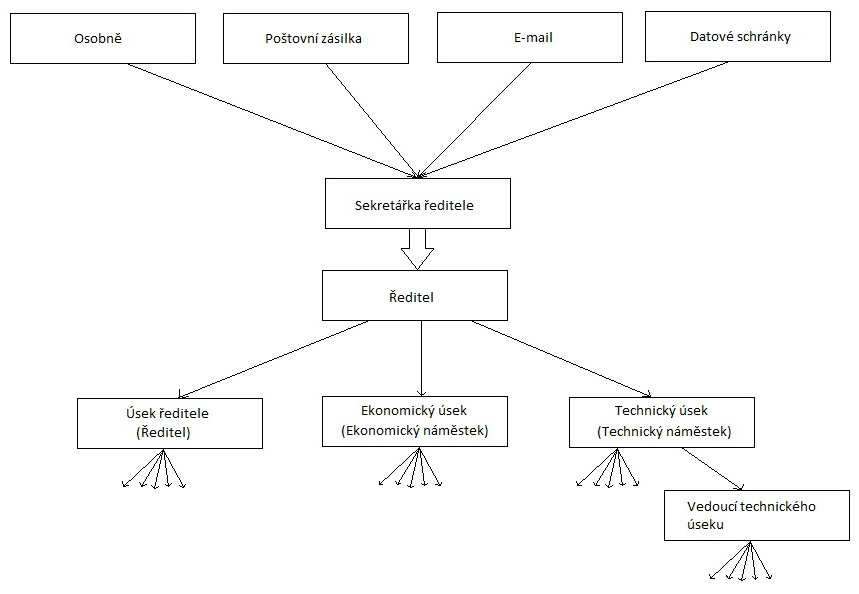
\includegraphics{tok_dokumentu.jpg} }
	\caption{Tok dokumentů v administrativě}
	\label{tok_dokumentu}
 \end{center}
\end{figure}

\subsection{Popis použitých postupů pro vytvoření modelu}

Zaměstnance společnosti modelujeme jako zařízení. To proto, že se tak skutečně chovají, zpracovávají požadavky po jednom za sebou.

Dokumenty modelujeme jako procesy, to zase odpovídá tomu, že při jejich zpracování zabírají zařízení a přitom mají nějakou dobu obsluhy.

Příchody transakcí do systému jsou modelovány událostmi, protože nemají trvání. Po\-ru\-cha zařízení je modelována jako proces, protože trvá určitou dobu.

\subsection{Popis původu použitých metod}

Během modelování jsme využívali znalosti získané na přednáškách a demosntračních cvičeních předmětu Modelování a simulace (IMS).

\newpage

% Kapitola 3 - 
\section{Koncepce}

Jako jednotku času v simulaci jsme zvolili jednu hodinu.
Modelovat \cite{ims-zakladni-pojmy} budeme pouze pracovní dobu zaměstnanců. Noci, víkendy a jiné události, kvůli kterým se nepracuje, jsou vynechány.
Tedy v čase 0 začíná první pracovní den a v čase 7.5 začíná druhý bez ohledu na to, zda mezi nimi byl např. víkend.

Příchody dokumentů do systému modelujeme procesy zvlášť pro příchozí klasickou poštu, elekteronickou poštu a příchody lidí osobně.
Elektronická pošta zahrnuje emaily společně s datovými schránkami, není potřeba je rozlišovat, protože jejich zpracování probíhá totožně.
Příchody lidí jsou modelovány příchody procesů v intervalech daných exponenciálním rozdělením se středem $T/n$ \cite{ims-rozlozeni}, kde $T$ je délka pracovního dne v ho\-di\-nách a $n$ průměrný počet příchodů denně.
Obdobně je modelován příchod dokumentů elektronicky, možnost příchodu elektronické zprvávy mimo pracovní dobu (např. v noci) zanedbáváme.

Ředitel společnosti je modelován zařízením s výlučným přístupem \cite{ims-zarizeni}, které je po dobu 6.5 hodiny obsazeno procesem s vyšší prioritou obsluhy,
který představuje všechny jeho pracovní povinnosti mimo administrativu, pro kterou je po zbylou 1 hodinu uvolněn.
Ne\-za\-bý\-vá\-me se, kdy přesně se administrativě ředitel věnuje, modelujeme pouze fakt, že se této činnosti věnuje pravidelně každý den danou dobu.

S pravděpodobností 30\% ředitel uvolněn pro administrativu není, tímto modelujeme fakt, že průměrně třikrát za dva týdny není pro administrativu k dispozici (3 z 10 pracovních dnů opovídá 30\% dnů).

Poruchy zařízení sekretářky jsou modelovány procesy s příchodem s exponenciálním rozdělením se středem 100 hodin. Předpokládáme že měsíc má 20 pracovních dní, tedy 150 pracovních hodin, během kterých se objeví průměrně 1.5 poruchy.

% Konceptuální model je abstrakce reality a redukce reality na soubor relevantních faktů pro sestavení simulačního modelu.
% Pokud některé partie reality zanedbáváte nebo zjednodušujete, musí to být zdůvodněno a videálním případě musí být prokázáno, že to neovlivní validitu modelu.
% Výsledek kapitoly: konceptuální (abstraktní) model s vyznačením relevantních faktů.

%  převzetí faktů do modelu
%  zdůvodněné provedené zjednodušení faktů
%  abstraktní popis modelu/programu

% Návod: koncepci vaší práce MUSÍ pochopit libovolný technik (a často i manažer...)

\newpage


% Kapitola 4 - 
\section{Architektura simulačního modelu/simulátoru}

Simulační model je implementován v jazyce C++ s využitím knihovny SIMLIB/C++.
% tohle je nejake moc strucne

% Nejméně zajímavá část. Obvykle se neuvádí.
% Rozeberte několik nejzajímavějších partií implementace
% Případná uživatelská příručka (spuštění programu, struktura výpisů, ...).
% O funkčnosti modelu musí přesvědčit kapitla 3.
% Není to referenční příručka!

% kapitola 4.1: Minimálně je nutno ukázat mapování abstraktního (koncept.) modelu do simulačního (resp. simulátoru). Např. které třídy odpovídají kterým procesům/veličinám a podobně. 
\subsection{Popis významu tříd simulačního modelu}

Příchozí dokumenty do systému v simulačním modelu jsou reprezezentovány instancemi třídy {\tt Dokument}.

Zaměstnance společnosti reprezentují zařízení {\tt reditel} - ředitel, {\tt sekretarka} - sekretářka, {\tt namestek\_tech} - technický náměstek,
{\tt namestek\_ekon} - ekonomický náměstek a {\tt vedouci\_tech} - vedoucí technického úseku.

Poruchy reprezentují události {\tt Porucha}.
Událost Email repreztuje příchod elektronického dokumentu, událost Lide společně s procesem {\tt Clovek} příchod lidí osobně.
Událost {\tt Postacka} reprezentuje příchod pracovnice pošty s poštou.

Procesy {\tt Reditel}, {\tt Namestek\_t} a {\tt Nameste\_e} modelují pracovní dobu ředitele a náměstků, kteří se nevěnují jen administrativě.


\newpage


% Kapitola 5 - 
\section{Podstata simulačních experimentů a jejich průběh}

Experimentováním s modelem chceme zjistit možné doby transakcí strávených v sys\-té\-mu. Pomocí těchto experimentů chceme ukázat strukturní a funkčí optimalizace systému toku dat v administrativě. Dále chceme ukázat pracovní vytíženost jednotlivých za\-měst\-nan\-ců při administrativních záležitostech. K tomu využijeme modelu a jeho pa\-ra\-met\-ri\-za\-ce, kdy například zvýšíme množství příchozí pošty, nebo poruchovost, nebo zvýšíme či snížíme pracovní výkonnost zaměstnanců.

% Experimentování musí mít předem zvolený a zdůvodněný řád, či postup
% 5.1 Postup experimentování a okolnosti studie
\subsection{Postup experimentování}
V modelu jsou již zaneseny zjištěné informace, jako například pracovní doba, množství příchozích transakcí a jejich časová rozložení, doba mezi poruchami, čas, který jednotliví pracovníci stráví nad jednou transakcí, pravděpodobnost, zda je ředitel v práci, atd. Tyto údaje jsou výrazným činitelem ovlivňujícím výsledek experimentu. Proto jsou zpočátku nastaveny na zjištěné a dále pro simulaci upravené hodnoty. Ty se budou pomocí experimentů dále upravovat tak, až bude model dostatečně podobný realitě. Poté se bude experimentovat pomocí změn těchto hodnot pro zjištění optimalizací systému.

Výsledkem experimentu bude histogram zobrazující dobu, kterou transakce stráví v systému. To znamená dobu do doručení transakce přímo adresátovi. Následná doba vyřizování příslušné transakce/dokumentu je v experimentech zanedbána, protože už se nejedná a studavanou problematiku. Z histogramu zjistíme, jaké jsou výsledky. Proč jsou výsledky takové, zjistíme z grafu závislostí vytíženosti jednotlivých pracovníků - kde se hromadí dokumenty, kdo je kdy zpracovává, atd. 

%
%
% POPIS GRAFU TADY ????
%
%

Experimenty budou modelovat průběh padesáti pracovních dnů.

% 5.2 Dokumentace jednotlivých experimentů
\subsection{Dokumentace jednotlivých experimentů}
\subsubsection{Experiment 1}
V tomto experimentu jsme parametry modelu nijak nemodifikovali, očekávali jsme, že výsledky budou odpovídat skutečnosti.
Oproti očekávání se většina transakcí dokončila velice rychle.
Histogram doby zpracování dokumentu v systému je na obrázku \ref{exp1_histogram}.
V období padesáti pracovních dnů systémem prošlo 2721 transakcí.
Ma\-xi\-mál\-ní doba trans\-ak\-ce strávené v systému byla 19.6 pracovních hodin.
Průměrná doba vyřízení transakce byla 8.01 pracovních hodin. Standardní odchylka 3.87 hodiny.

Z časového průběhu délek front jednotlivých zaměstnanců, jsme zjistili nedostatek mo\-de\-lu.
Příchozí dokumenty se zdržely zejména u ředitele, na jednotlivích úsecích firmy se již takřka vůbec nezdržely a téměř okamžitě putovaly ke svým adresátům.
To bylo způsobeno tím, že náměstci byli celou dobu k dispozici k práci na administrativě a nevznikalo u nich zpoždění ve frontách.
Ve skutečnosti je ale administrativa, podobně jako u ředitele, jen část náplně jejich pracovní doby.

V následujících experimentech budeme pracovat s upraveným modelem, ve kterém se tento nedostatek neprojeví.
Oba náměstci se po většinu své pracovní doby budou věnovat jiným pracovním povinnostem a administrativě  
pouze hodinu během jednoho pracovního dne jako ředitel.

\begin{figure}[ht]
 \begin{center}
    \scalebox{0.4}{ 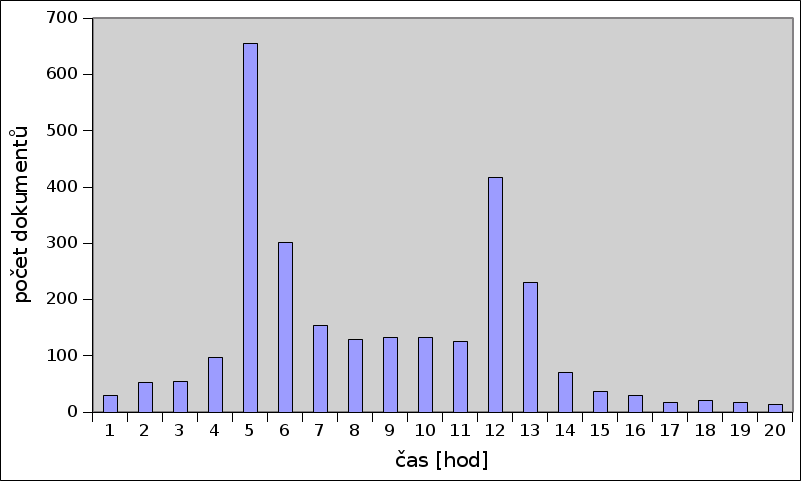
\includegraphics{../experimenty/ex1-histogram.png} }
    \caption{1. experiment - histogram doby zpracování dokumentu}
    \label{exp1_histogram}
 \end{center}
\end{figure}

% 5.3 Závěr experimentů
% Co bylo experimentováním zjištěno
% Jaké chyby v modelu byly odstraněny (oproti původním předpokladům ... došlo ke změně koncepce ... protože ..
\newpage


% Kapitola 6 - 
\section{Shrnutí simulačních experimentů a závěr}

% Jednoznačná odpověď na prvotní otázku studie.
%  Studií provedenou na našem modelu bylo jednoznačně prokázáno/vyvráceno, že ...
%  V rámci experimentů bylo zjištěno, že průměrné zatížení ... je ...
%  Z experimentů vyplývá jednoznačné doporučení, aby provozovatel ... rozšířil výrobu o ...
%  Ze statisticky zpracovaného měření v terénu plyne, že proces příchodů ... se řídí normálním rozložením se středem a ....
% • Na přiložených demo-příkladech jsme ověřili funkčnost ...

\newpage

% Reference
%\renewcommand{\refname}{Literatura}
%\cite{voj,has}
\begin{thebibliography}{99}

\bibitem{ims-sho} P. Peringer.
\textit{Modelování a simulace: Systémy hromadné obsluhy.}
Dostupné z: \textless https://www.fit.vutbr.cz/study/courses/IMS/public/prednasky/IMS.pdf\textgreater.
Strana 139.

\bibitem{ims-zakladni-pojmy} P. Peringer.
\textit{Modelování a simulace: Zakladni pojmy.}
Dostupné z: \textless https://www.fit.vutbr.cz/study/courses/IMS/public/prednasky/IMS.pdf\textgreater.
Strana 7-8.

\bibitem{ims-chovani-systemu} P. Peringer.
\textit{Modelování a simulace: Chování systému.}
Dostupné z: \textless https://www.fit.vutbr.cz/study/courses/IMS/public/prednasky/IMS.pdf\textgreater.
Strana 24.

\bibitem{ims-rozlozeni} P. Peringer.
\textit{Modelování a simulace: Nekterá často používaná rozložení.}
Dostupné z: \textless https://www.fit.vutbr.cz/study/courses/IMS/public/prednasky/IMS.pdf\textgreater.
Strana 90-99.

\bibitem{ims-zarizeni} P. Peringer.
\textit{Modelování a simulace: ??? Zařízení s vylučným přístupem ???.}
Dostupné z: \textless https://www.fit.vutbr.cz/study/courses/IMS/public/prednasky/IMS.pdf\textgreater.
Strana ???.

%\bibitem{voj} T. Vojnar. Towards Formal Analysis and Verification
%over State Spaces of Object-Oriented Petri Nets. PhD. thesis,
%Brno University of Technology, Brno, Czech Republic, 2001.

\end{thebibliography}

\end{document}
